\chapter{Foundations}
\label{cha:foundations}

\section{Use Cases Motivation}

The company BestRental wants to develop a monitoring solution for its BestRentalPoC system
to collect metrics that are meant to assist the company in operating the BestRentalPoC.
The system will be operated by QA Engineers, system operators, and a project manager.
Before developing the monitoring solution, the team tasked with developing the solution,
interview the different roles to find out how they will use the solution
and what their tasks and responsibilities are.
QA Engineers are responsible for the reliability of BestRentalPoC.
To ensure the reliability of the system, they want to know when requests to the system fail and
trigger errors, so that they can fix them.
For them to better understand errors, they want to know how often errors occur and from which services,
inside of BestRentalPoC, they originate.
The system operators run the BestRentalPoC. They need to make sure that at any point in time
BestRentalPoC has enough instances of all of its services available to serve all incoming requests.
Because BestRental wants to operate profitably, they can't just create as many instances as they like,
and they need to shut down instances when they are not needed.
To assist them with their task, they want to know how high the resource usage of each instance is
and how many requests are coming into the system. The resources that they want to track for each
instance are the instance's CPU and memory usage.
The project manager's yearly bonus is tied to how profitable the BestRentalPoC operates.
To ensure that he gets his bonus, the project manager wants to track the operating costs of the complete system.
Additionally, he needs to how high the operating costs of each service are, so that he can
allocate development time to increase the efficiency of a service, making it more profitable.
After the interviews, the development notes that all types of users of the monitoring solution
want to be able to do five different things.
Firstly, they want to be able to create a dashboard for a metric that displays its current and historic values.
When viewing a dashboard they also want to be able to run queries on the metric to, for example, get
its value at a specific point in time.
Because the users can't constantly watch all of their dashboards, they want to be able to create
alerts for a metric that will be triggered when the metric exceeds a set value.
When a metric exceeds a value set for an alert, the users want to receive the alert so that they can act on it.
The developers also know that the solution needs to be able to do three main things to accomplish
the requested features.
Firstly, the solution needs to collect metrics from BestRentalPoC,
it then needs to analyze the collected data, and lastly, it needs to conditionally send out alerts
for metrics.

\section{Use Case}

\begin{figure}[h]
	\centering
	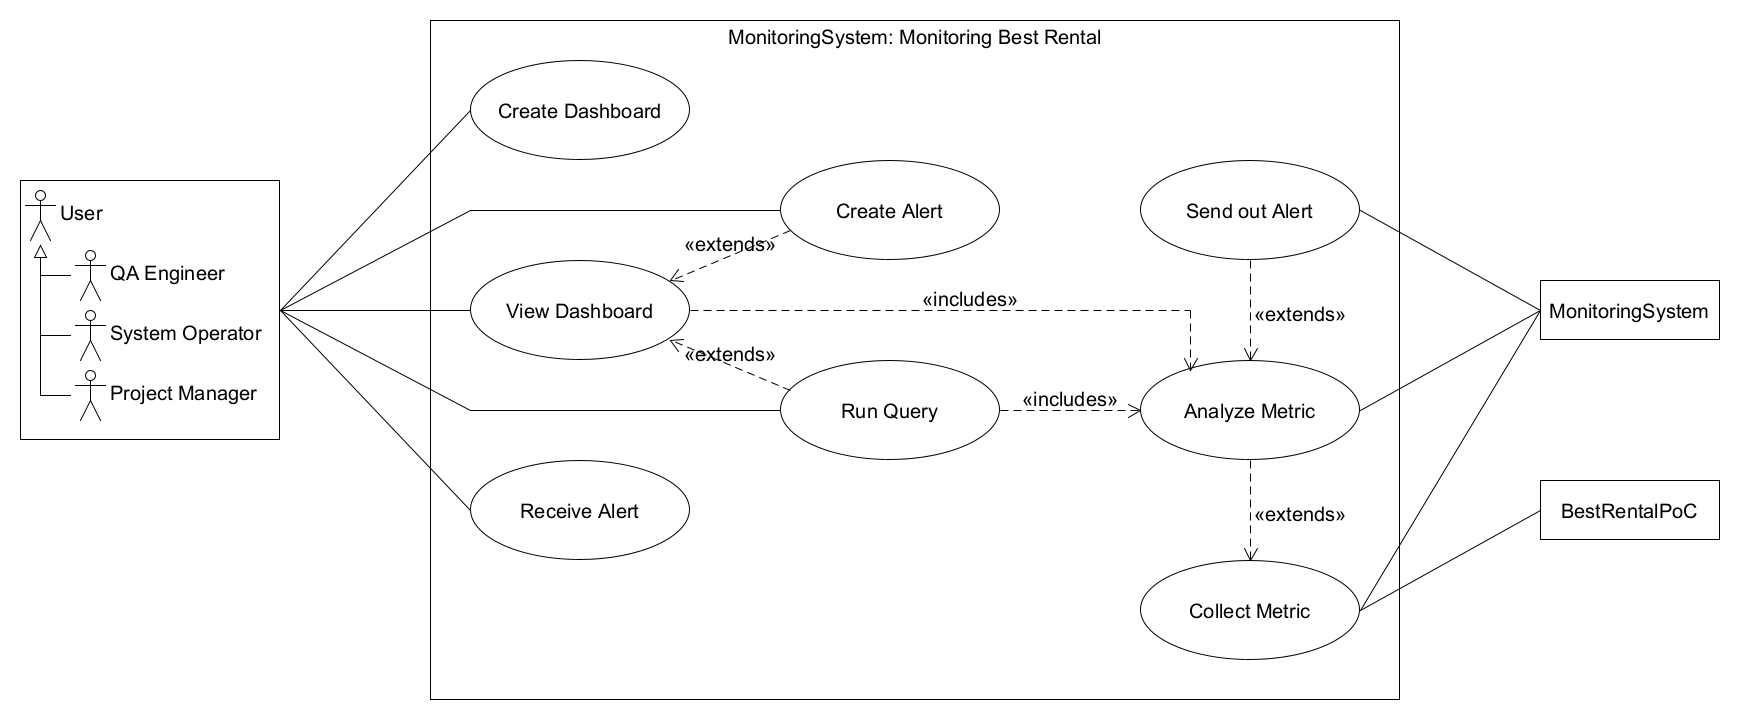
\includegraphics[width=\textwidth]{figures/use_case_monitoring_bestrental.png}
	\caption{Use Case: Monitoring BestRental}
	\label{fig:use_case_monitoring_best_rental}
\end{figure}

\vspace{0.5cm}
\begin{lstlisting}[caption = {Use Case Description: Monitoring BestRental}, label = {lis:use_case_description_monitoring_bestrental}, style = kit-cm, language=] 
Title: User monitors BestRentalPoC

Primary Actors: User
Secondary Actors: MonitoringSystem

Preconditions:  
- The user has a valid account for the monitoring system
- The monitoring system is configured to collect Metric X
Postconditions:  
- The monitoring system has a dashboard for Metric X
- The monitoring system has an alert set up for Metric X

Flow:
1. The user logs into the monitoring system
2. The user creates a new dashboard for Metric X
3. The user views the dashboard for Metric X
4. The user creates an alert for Metric X
5. The user receives an alert for Metric X
6. The user runs a query on Metric X
7. The user logs out of the monitoring system

Alternative flows:
5a. The alert for Metric X is not triggered
  5a1. The user does not receive an alert for Metric X
	
Information Requirements: 
- Metric X
- Value that Metric X must exceed for the alert to be triggered
\end{lstlisting}

\vspace{0.5cm}
\begin{lstlisting}[caption = {Use Case Description: Monitoring BestRental}, label = {lis:use_case_description_monitoring_bestrental}, style = kit-cm, language=] 
Title: MonitoringSystem monitors BestRentalPoC

Primary Actors: MonitoringSystem
Secondary Actors: BestRentalPoC

Preconditions:  
- The monitoring system is configured to collect Metric X
- The monitoring system has an alert set up for Metric X
Postconditions:  
- An alert for Metric X has been sent out

Flow:
1. The monitoring system collects the latest values for Metric X from BestRentalPoC
2. The monitoring system analyzes the values for Metric X
3. The monitoring system sends out an alert for Metric X

Alternative flows:
3a. The alert for Metric X is not triggered
  5a1. The monitoring system does not send out an alert
	
Information Requirements: 
- Metric X
- Value that Metric X must exceed for the alert to be triggered
\end{lstlisting}